\begin{figure}[h!]
    \begin{center}
        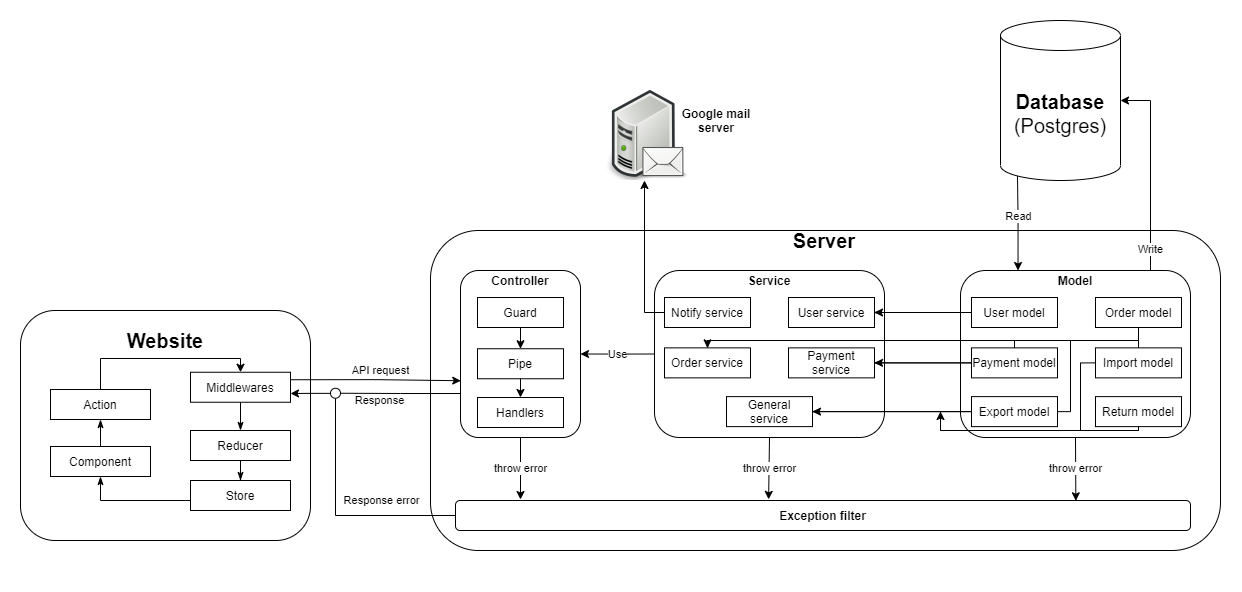
\includegraphics[width=14cm]{Image/Technical/architecture.png}
        \caption{Kiến trúc hệ thống}
        \label{architecture}
    \end{center}
\end{figure}

Kiến trúc của hệ thống được thiết kế đơn giản như Hình \ref{architecture} bao gồm các thành phần sau:
\subsubsection{Website (front-end)}
\begin{itemize}
    \item Component: chứa các view hiển thị cho người dùng.
    \item Action: nhận các sự kiện mà người dùng thực hiện.
    \item Middlewares và Reducer xử lí các sự kiện của người dùng, các dữ liệu từ server trả về để tính toán trả về state mới.
    \item Store: lưu tất cả state của ứng dụng.
\end{itemize}
\subsubsection{Server (back-end)}
\begin{itemize}
    \item \textbf{Controller}: nhận request trực tiếp từ người dùng, request đi vào controller sẽ đi qua ba bước (có thể có ngoại lệ) cơ bản bao gồm:
    \begin{itemize}
        \item Guard: xác thực người dùng, xem người dùng có phải là người dùng của hệ thống hay không, nếu đúng, nó có thể xét tiếp vai trò của người dùng đó.
        \item Pipe: xác nhận dữ liệu truyền từ người dùng có đúng định dạng, kiểu. Ngoài ra, nó còn thực hiện chuyển đổi dữ liệu trong một số trường hợp.
        \item Handlers: xử lý request của người dùng, điều khiển, gọi các Service tương ứng để xử lý, và phản hồi kết quả cho người dùng. Một handler có thể gọi cùng lúc nhiều service.
    \end{itemize}
    
    \item \textbf{Services}: nhận yêu cầu từ controller để xử lý một tác vụ nào đó và trả về kết quả. Một service cũng có thể gọi và được gọi từ các service khác. Một service có thể là chủ của một hoặc nhiều model. Service sử dụng model để thao tác với cơ sở dữ liệu chứ không trực tiếp làm việc này.
    
    \item \textbf{Models} là thành phần thao tác trực tiếp với CSDL. Một model ánh xạ chính xác một quan hệ từ cơ sở dữ liệu và các ràng buộc liên quan. Các model có mối liên hệ với nhau bằng mối liên hệ của đối tượng.
    
    \item \textbf{Exception Filter} được dành riêng cho việc bắt các lỗi exception và phản hồi lỗi về cho người dùng. Việc chỉ định vai trò này cho một mình Exception Filter thể hiện rõ tính module hoá.

\end{itemize}
Các lớp thành phần ở trên độc lập với nhau, không xung đột lẫn nhau. Mỗi lớp cần thông tin sẽ gọi về lớp thấp hơn, cũng như cung cấp thông tin cho lớp cao hơn.

\subsubsection{Database}
Cơ sở dữ liệu là nơi lưu trữ tất cả dữ liệu cần thiết của ứng dụng, đảm bảo có thế truy cập bất cứ lúc nào và bất cứ đâu. Các quan hệ trong cơ sở dữ liệu được ánh xạ và làm việc trực tiếp với lớp Models. Cơ sở dữ liệu sẽ thực hiện mọi câu lệnh SQL để query dữ liệu, update dữ liệu. tạo mới dữ liệu,...